\documentclass[10pt]{beamer}


\mode<presentation> 
{
  \usetheme{Diku}
  \beamertemplatenavigationsymbolsempty
  \setbeamercovered{invisible}
%  \setbeamercovered{transparent}
}



% \mode<presentation> 
% { \usetheme[nat,dogma]{Frederiksberg} }

% \usepackage[danish]{babel}
\usepackage[latin1]{inputenc}
\usepackage{times}
\usepackage[T1]{fontenc}
\usepackage[english]{babel}
\usepackage{hyperref}
\usepackage{animate}
%\usepackage{multimedia}
\usepackage{francois-preamble}
\usepackage{multirow}

\usepackage{multirow}
%\usepackage{movie15}

\newcommand{\cc}{{c\!\!,}}
\newcommand{\degr}[1]{{{#1}^\circ}}

\title{Vision and Image Processing:\\ Camera Models}

\author[S. Olsen] % (optional, use only with lots of authors)
{S�ren Olsen}

\institute[DIKU] % (optional, but mostly needed)
{
  Department of Computer Science\\
  University of Copenhagen
}

\date[2014-15 B2] % (optional, should be abbreviation of conference name)
% {Research Presentation, Diku 2006}


% Insert page numbers
\pagenumbering{arabic}
\setbeamertemplate{footline}{\hspace{5pt}\insertpagenumber\vspace{10pt}}



\definecolor{gold}{rgb}{0.95,0.83,0.0}
\definecolor{orange}{rgb}{0.95,0.7,0.0}
% \definecolor{backblue}{rgb}{0.93,0.94,0.99}
\definecolor{backblue}{rgb}{0.95,0.94,0.99}
\setbeamercolor*{background canvas}{bg=backblue} 



\newcommand{\myemph}[1]{{\color{blue}{#1}}}
\newcommand{\intrg}[1]{\int_{{#1}=-\infty}^\infty}
\newcommand{\intRR}{\int_{-\infty}^\infty}

\AtBeginSection[]
{
  \begin{frame}<beamer>{Outline}
    \tableofcontents[currentsection,currentsubsection]
  \end{frame}
}

\begin{document}
\maketitle

% would be cool with more images showing applications


%-------------------------------------------------------------------
%   Start slides
%-------------------------------------------------------------------


%----------------------------------------------
\begin{frame}
  \frametitle{Plan for today}
  \begin{itemize}
  \item Introduction to Camera Models, specifically the pinhole model
    and the perspective transformmation \\[3mm]
  \item Vanishing points and vanishing lines \\[3mm]
  \item Projections, projective geometry, homographies \\[3mm]
  \item Camera matrices and parameters
  \end{itemize}
\end{frame}




% ----------------------------------------------------
\begin{frame}
  \frametitle{Cameras and projections}
  \begin{center}
    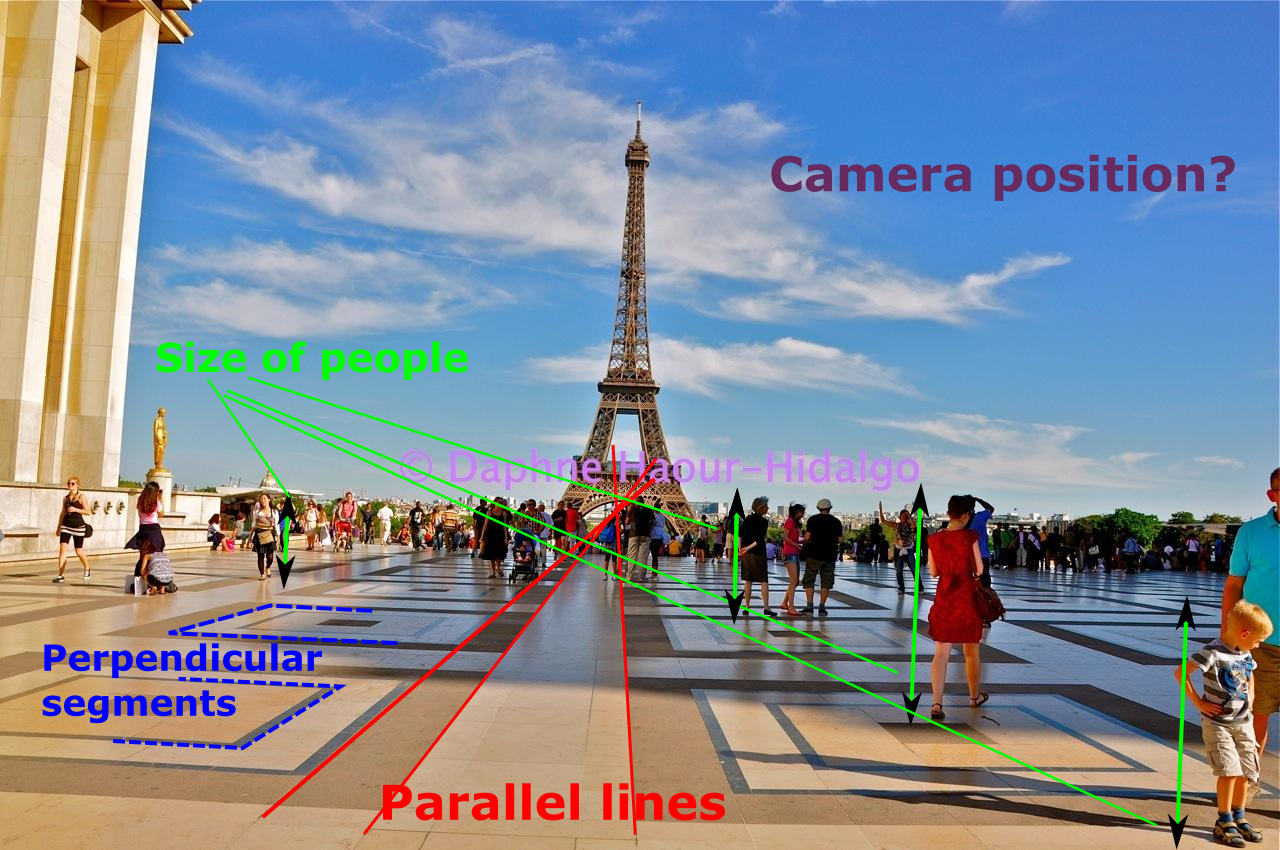
\includegraphics[width=\textwidth]{IMAGES/trocadero_annotations}
  \end{center}
\end{frame}


% ----------------------------------------------------
% \begin{frame}
%  \frametitle{Questions}
%  Previous picture raises some questions about:\vfill
%  \begin{itemize}
%   \item Lines?
%   \item Parallelism?
%   \item Angles / orthogonality?
%   \item Sizes?
%   \item Camera position / Horizon?\vfill
%   \end{itemize}
%   What happens when you take a picture (or Daphn{\'e} Haour-Hidalgo in the previous case :-))
% \end{frame}


% \section{The Pinhole Camera}


% ----------------------------------------------------
% \begin{frame}
%  \frametitle{Getting an Image -- I}
%  \begin{center}
%    \includegraphics[width=0.55\textwidth]{FIGURES/oliphantnopinhole}
%  \end{center}
%  Many rays emanating from the same position touch the image sensitive
%  array at many location: big blur!
% \end{frame}

% ----------------------------------------------------
% \begin{frame}
%  \frametitle{Getting an Image -- II}
%  \begin{center}
%    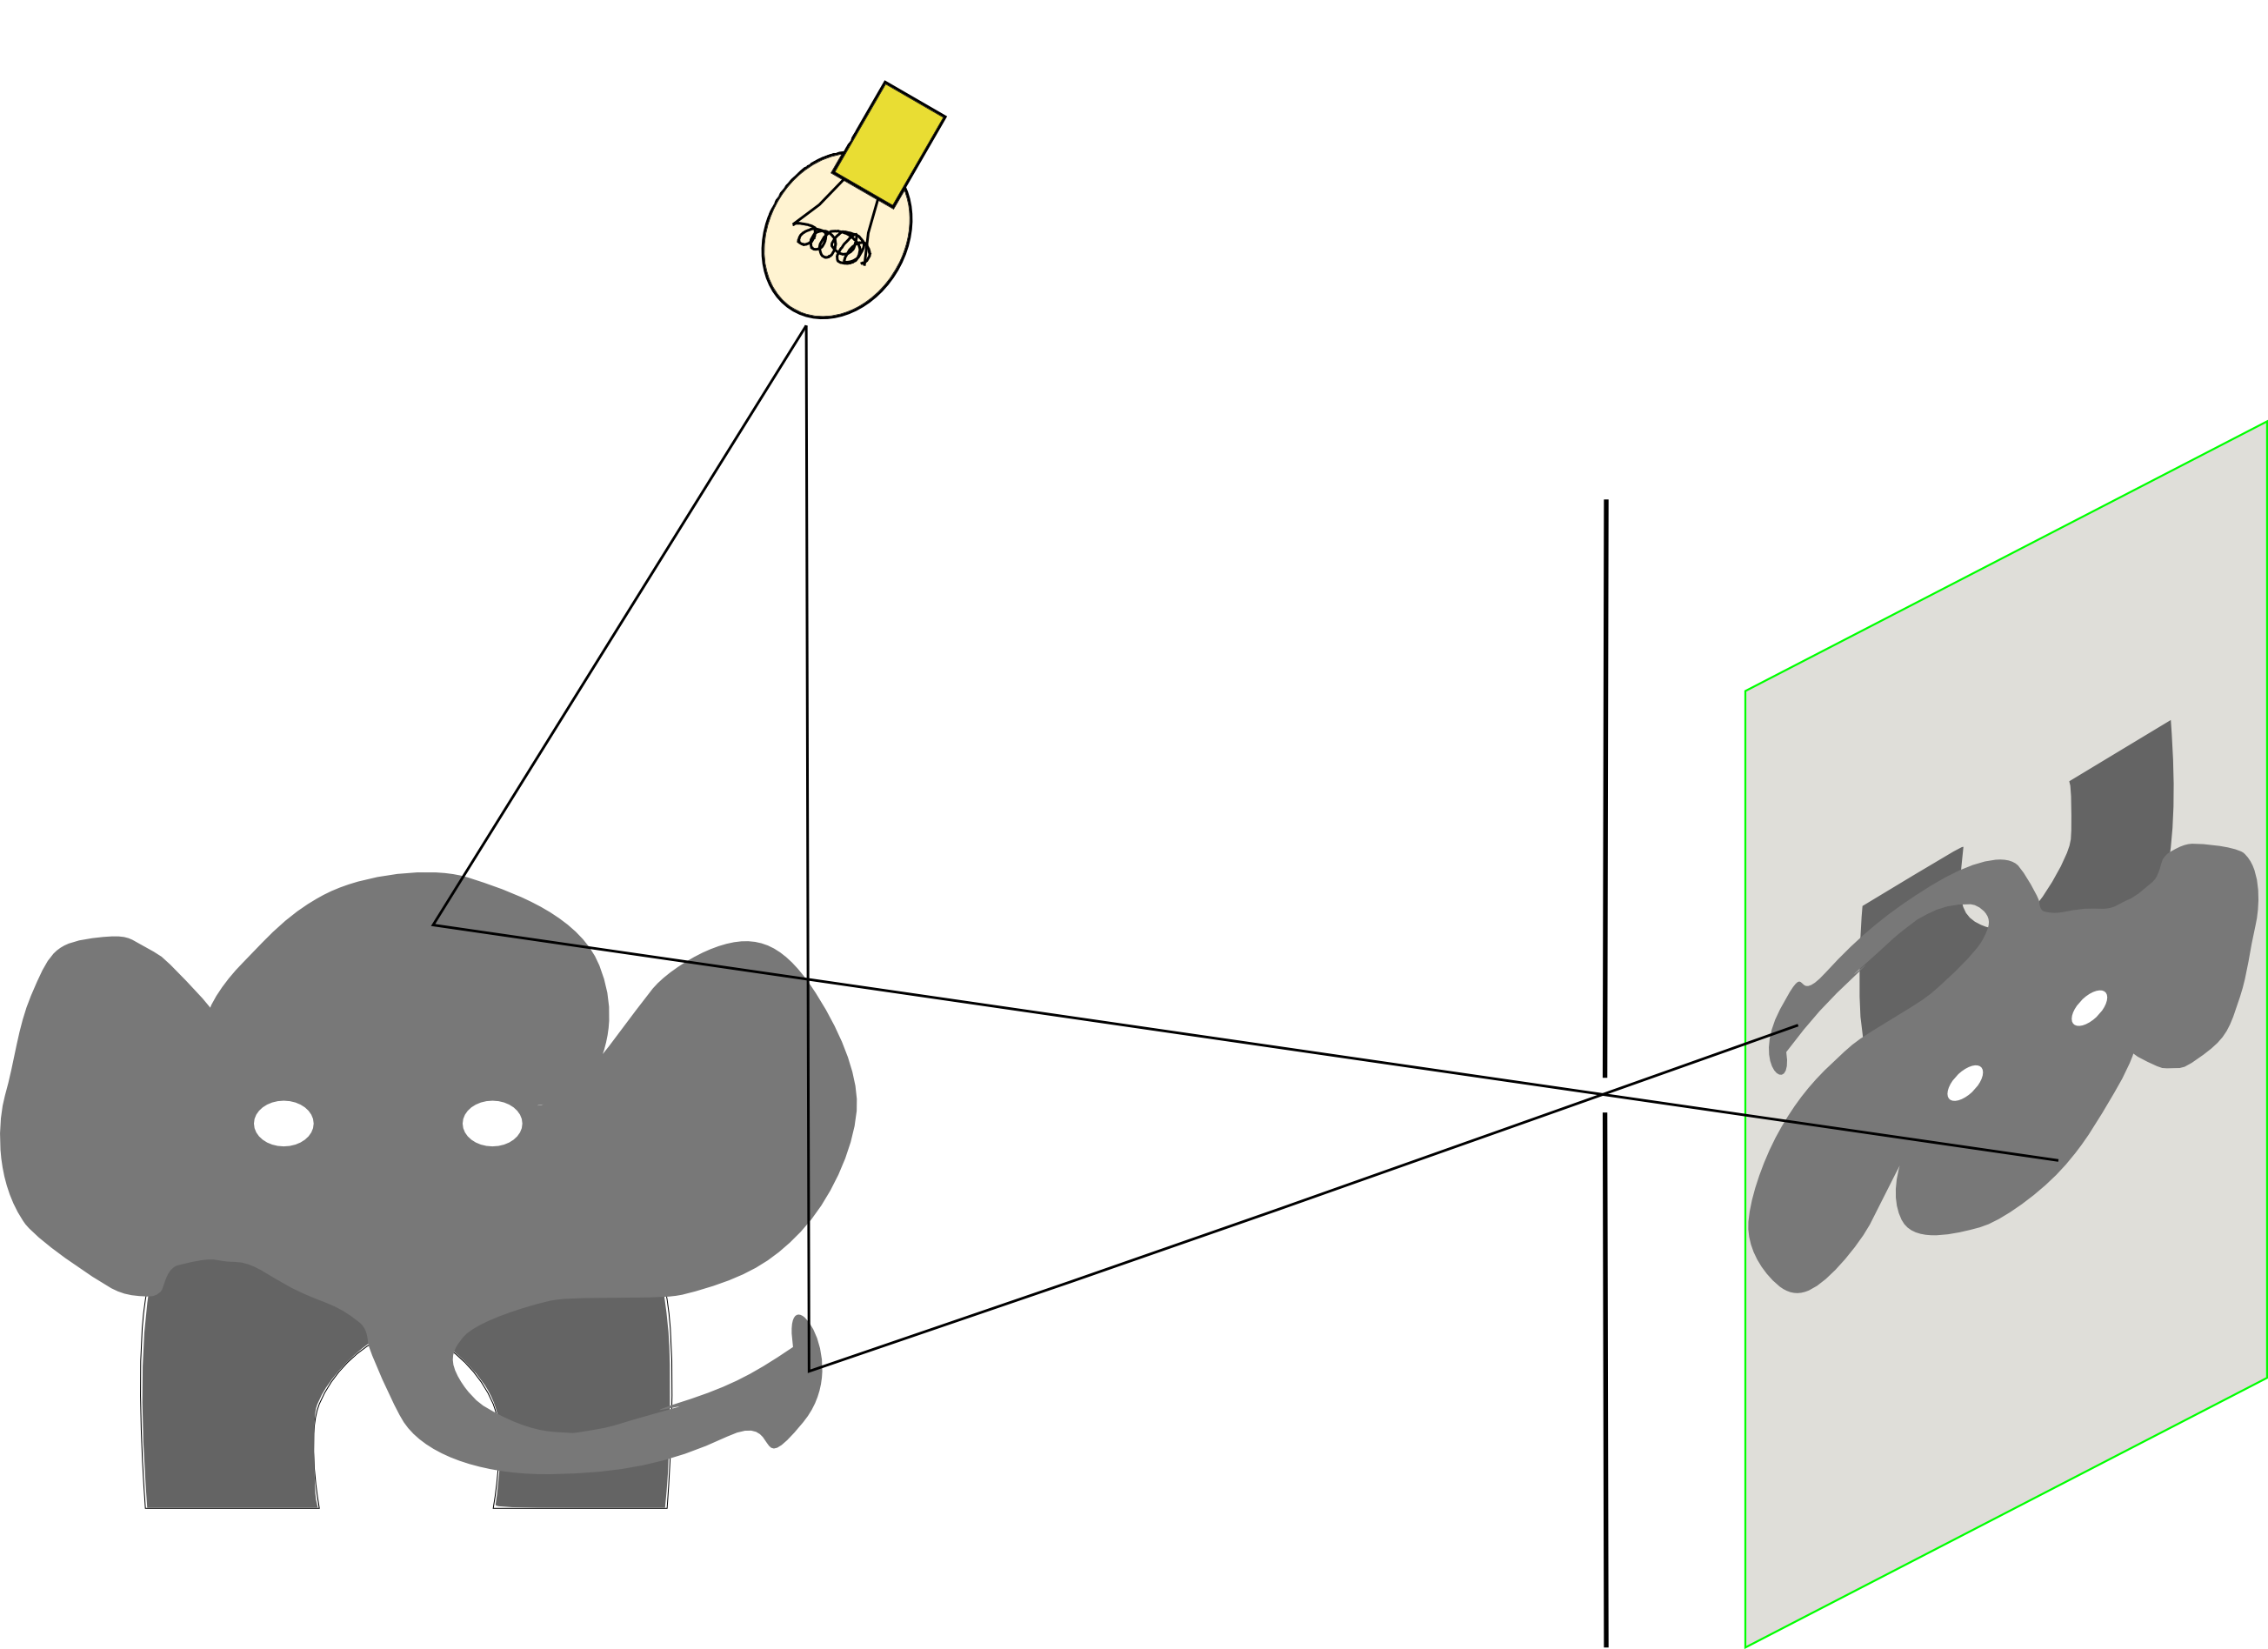
\includegraphics[width=0.65\textwidth]{FIGURES/oliphantpinhole}
%  \end{center}
%  Filtering the rays via a pinhole: get an (inverted) image. Principle
%  of the \myemph{Camera Obscura} (dark room).
% \end{frame}

% \section{A bit of History}


% ----------------------------------------------------
\begin{frame}
  \frametitle{Camera Obscura}
  \begin{center}
    \begin{tabular}[h]{cc}
      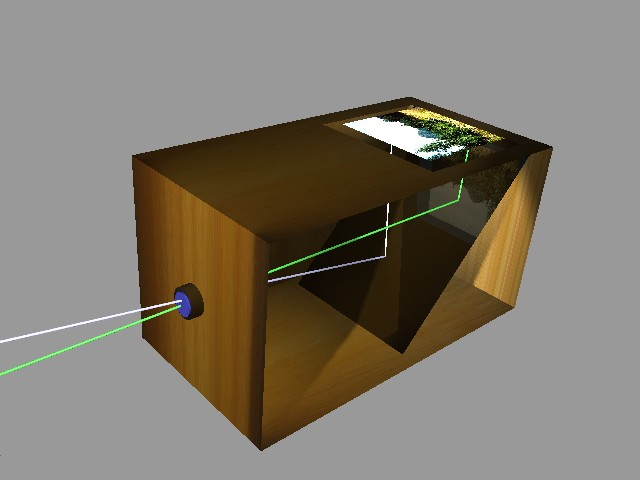
\includegraphics[width=0.4\textwidth]{IMAGES/WMCamera_obscura_box} &
      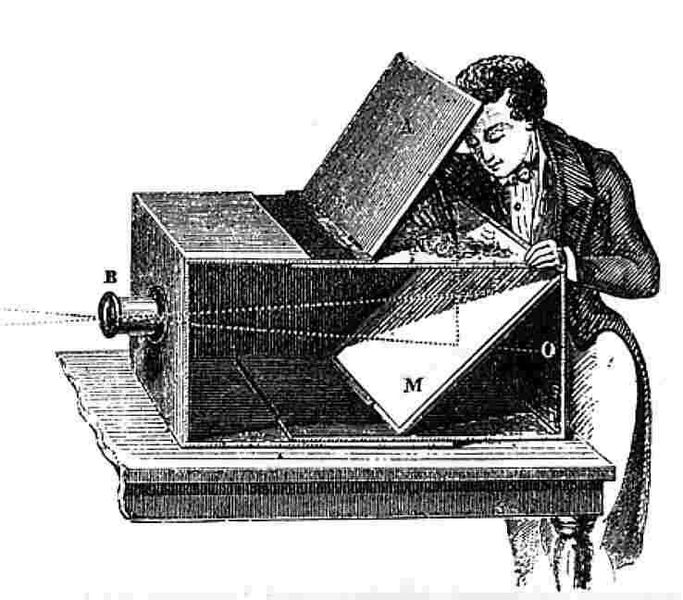
\includegraphics[width=0.4\textwidth]{IMAGES/WMCameraObscura18thCentury}\\
      Principle of Camera Obscura & 18th Century Camera Obscura
    \end{tabular}
  \end{center}
  \begin{itemize}
  \item Known from old chines writings
  \item Mentioned by Aristotle
  \item Plaque with photosensitive material: Photographic camera!
  \end{itemize}
\end{frame}


% ----------------------------------------------------
\begin{frame}
  \frametitle{The Very First Photography, 1826}
  \begin{center}
    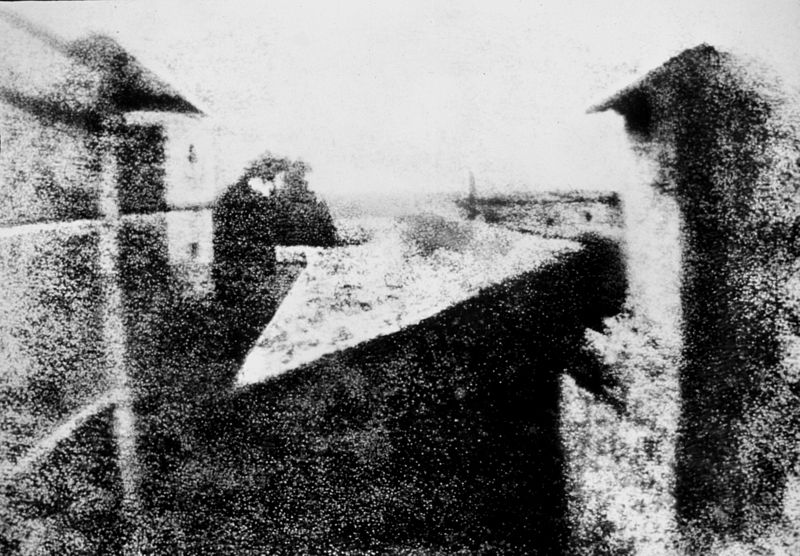
\includegraphics[width=0.8\textwidth]{IMAGES/WindowLegrasNiepce}
  \end{center}
  J.N. Ni�pce, View from the window at Le Gras,
  Saint Loup de Varennes, France -- Now at University of Texas at
  Austin.
\end{frame}




% ----------------------------------------------------
\begin{frame}
  \frametitle{The pin-hole camera}
  \begin{center}
    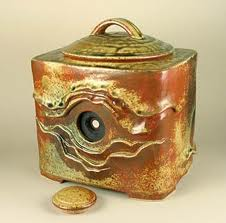
\includegraphics[width=0.4\textwidth]{IMAGES/pinholecamera.jpg}
    \hspace{2mm}
    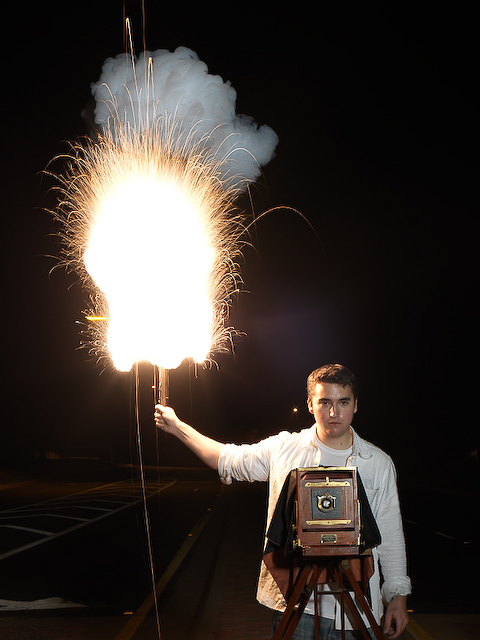
\includegraphics[width=0.4\textwidth]{IMAGES/magnesiumbomb.jpg}
  \end{center}
  Mangnesium light was used to make light enough enter the pin-hole box.
\end{frame}


% ----------------------------------------------------
% \begin{frame}
%    \begin{center}
%    \frametitle{The Pioneers}
%    \begin{tabular}[h]{ccc}
%      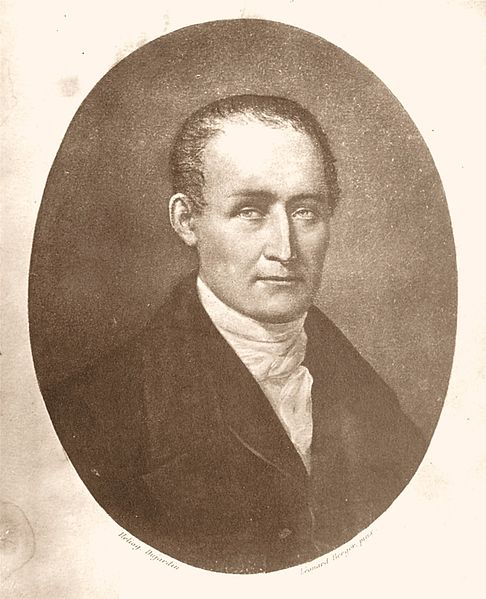
\includegraphics[width=0.3\textwidth]{IMAGES/JNNiepce} &
%      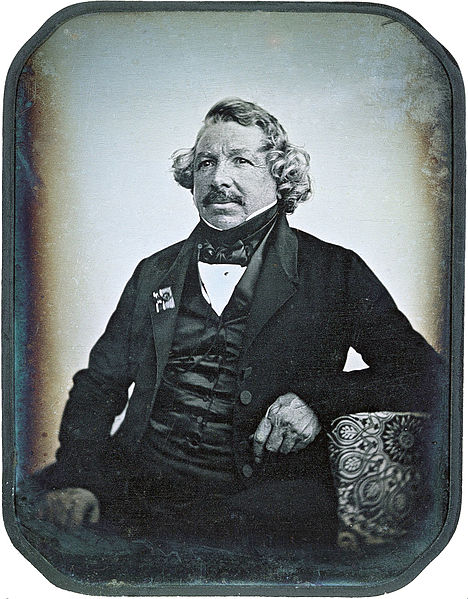
\includegraphics[width=0.3\textwidth]{IMAGES/LDaguerre} &
%      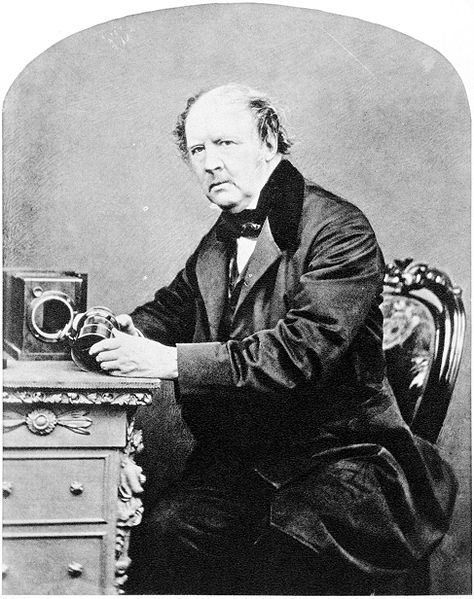
\includegraphics[width=0.3\textwidth]{IMAGES/HFTalbot} \\
%      J. Nicéphore Nièpce & Louis Daguerre & Henri F. Talbot
%    \end{tabular}
%  \end{center}
% \end{frame}


% ----------------------------------------------------
% \begin{frame}
%  \frametitle{Now...}
%  \begin{center}
%    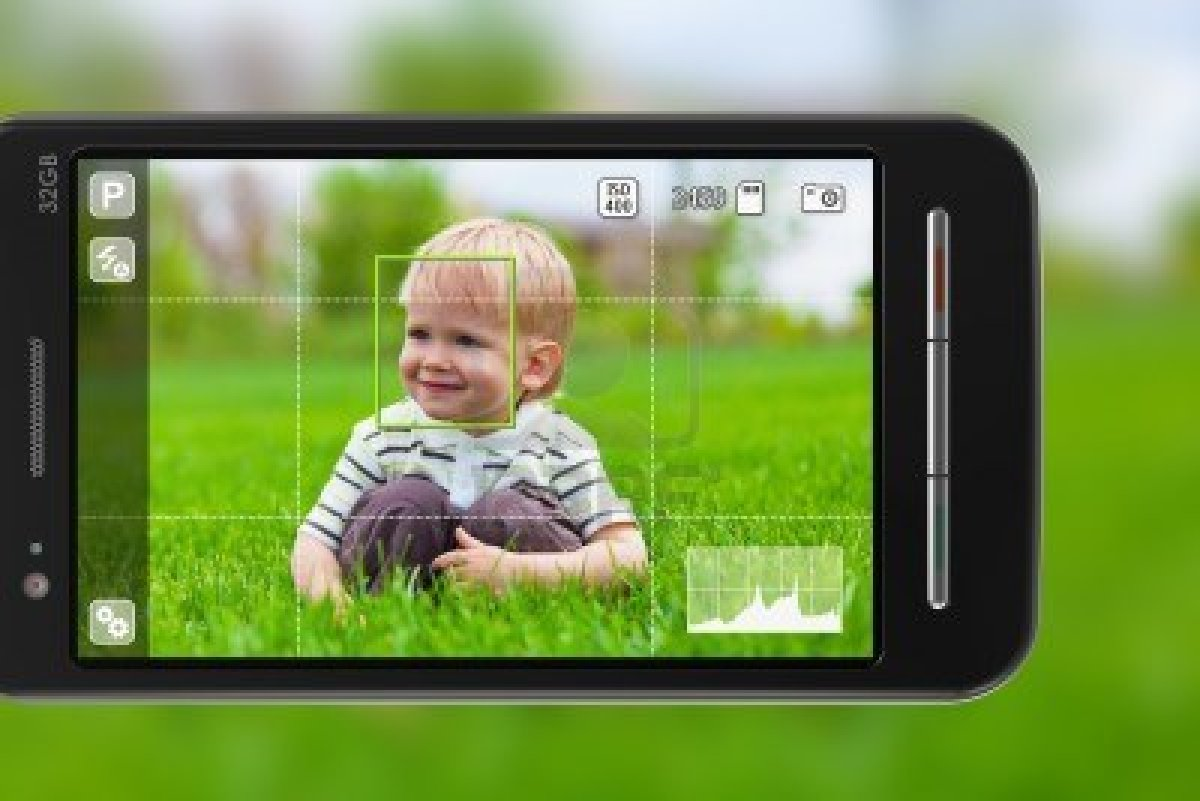
\includegraphics[width=0.8\textwidth]{IMAGES/smartphonecamera}
%  \end{center}
% \end{frame}



% \section{Projection}

% ----------------------------------------------------
\begin{frame}
  \frametitle{The Pinhole Camera Model}
  \begin{center}
    \includegraphics[width=0.9\textwidth]{FIGURES/coproj}
  \end{center}
  \begin{itemize}
  \item $f$ is the focal length,
  \item $O$ is the camera center.
  \end{itemize}
\end{frame}


% ----------------------------------------------------
\begin{frame}
  \frametitle{Projection is Tricky!}
  \begin{center}
    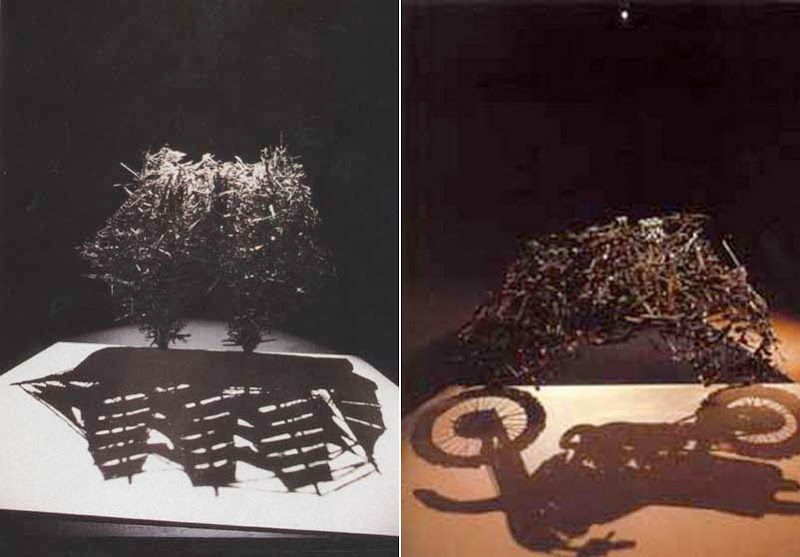
\includegraphics[width=0.8\textwidth]{IMAGES/shigeoFukuda}
  \end{center}
  Some illusions from Shigeo Fukuda. 
\end{frame}



% ----------------------------------------------------
\begin{frame}
  \frametitle{Perspective Effects}
  Remember from Kim's first lecture
  \begin{center}
    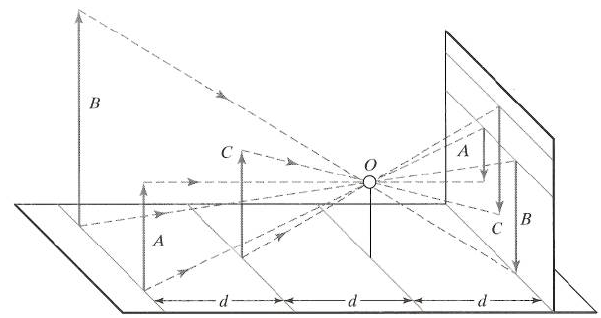
\includegraphics[width=0.9\textwidth]{FIGURES/fp131}
  \end{center}
  Far objects appear smaller that close ones.
\end{frame}


% ----------------------------------------------------
\begin{frame}
  \frametitle{Perspective Effects}
  Remember from Kim's first lecture again
  \begin{center}
    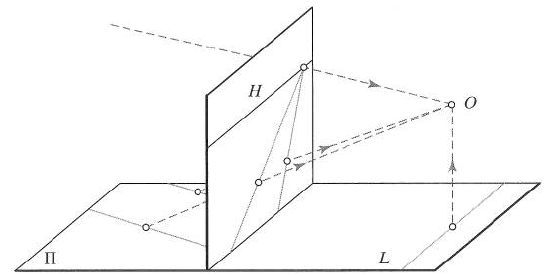
\includegraphics[width=0.9\textwidth]{FIGURES/fp132}
  \end{center}
  Images of parallel lines intersect at the horizon (virtual image plane).
\end{frame}



% ----------------------------------------------------
% \begin{frame}
%  \frametitle{Stereo disparity}
%  \begin{center}
%    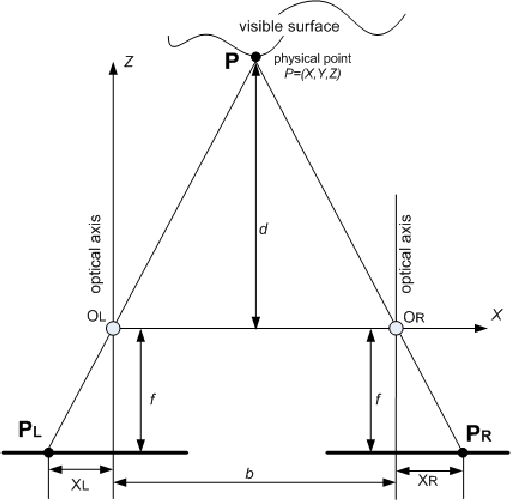
\includegraphics[width=0.9\textwidth]{MyImages/Stereo.png}
%   \end{center}
%  \begin{itemize}
%   \item Let the projection of $P$ on the baseline $O_L O_R$ be divided
%    in distances $A$ and $B$ and notice the two pairs of similar
%   triangles.
%  \item We have that $Z/A = f/x_L$ and that $Z/B = f/(-x_R)$.  Then
%    $$
%     b = A + B = Z \frac{x_L}{f} + Z \frac{-x_R}{f} = 
%    \frac{Z}{f} (x_L - x_R) = \frac{Z}{f}d
%    $$
%    where $d$ is the \myemph{disparity}.  Rewriting:
%   $$
%     Z = \frac{bf}{d}
%    $$
%   \end{itemize}
% \end{frame}


% ----------------------------------------------------
\begin{frame}
  \frametitle{Projection Equations}
  \begin{center}
    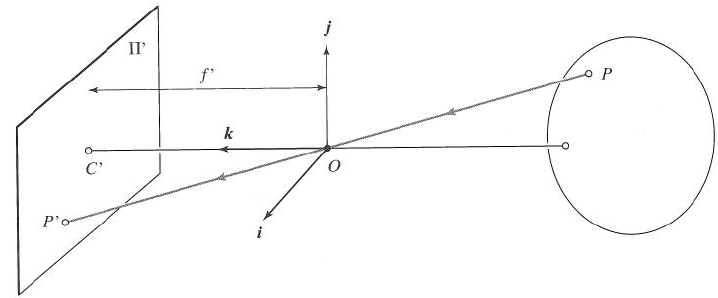
\includegraphics[width=0.9\textwidth]{FIGURES/fp14}
  \end{center}
  \begin{itemize}
    \item  $P (x,y,z)$, $P' (x',y',z')$. $P'$ in the image plane $\implies z' = f$
    \item Remember: similar triangles:
    $$
     x' = f\frac{x}{z},\quad y' = f\frac{y}{z}
    $$
  \end{itemize}
\end{frame}


% ----------------------------------------------------
\begin{frame}
  \frametitle{Lost in projection}
    \begin{center}
    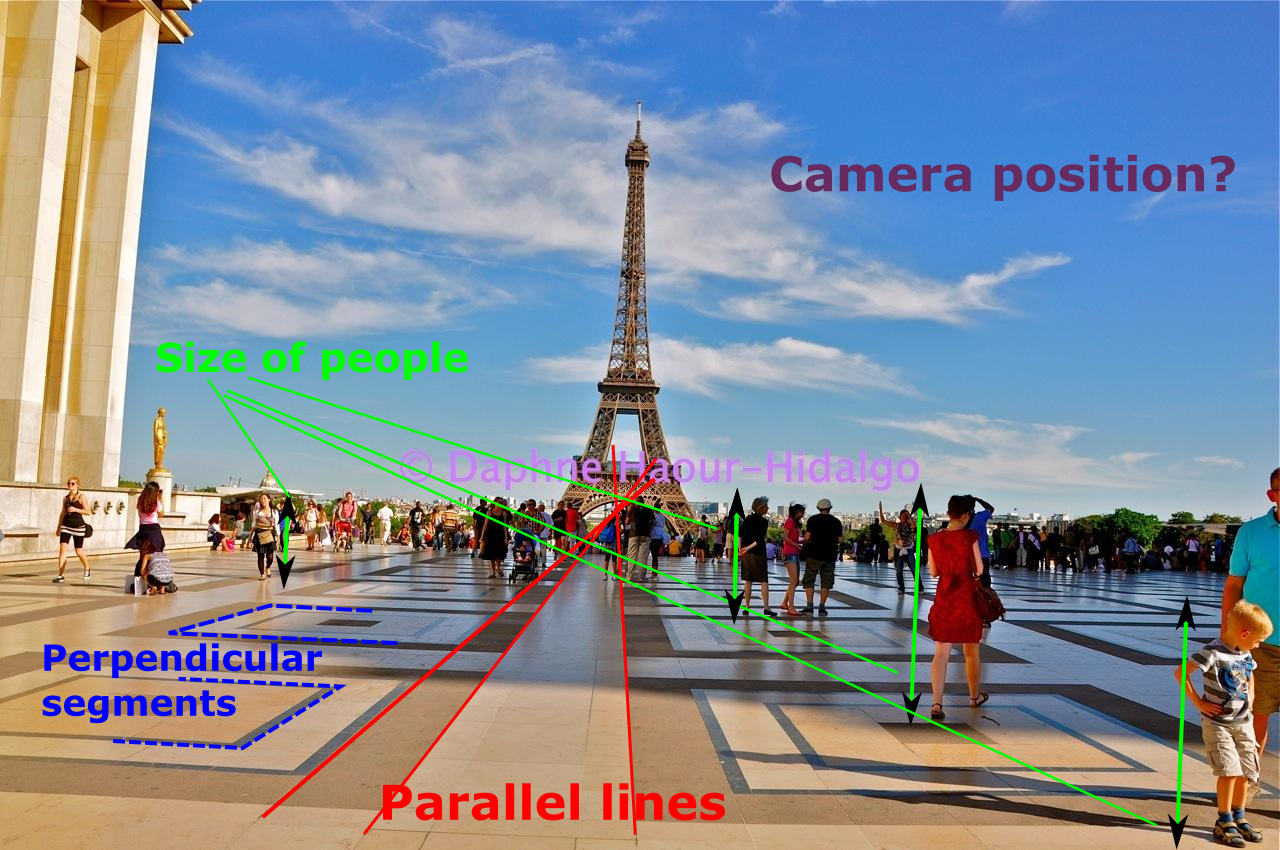
\includegraphics[width=0.8\textwidth]{IMAGES/trocadero_annotations}
  \end{center}
  Depth, Angles, size, parallelism.
\end{frame}


% ----------------------------------------------------
\begin{frame}
  \frametitle{Preserved by projection}
    \begin{center}
    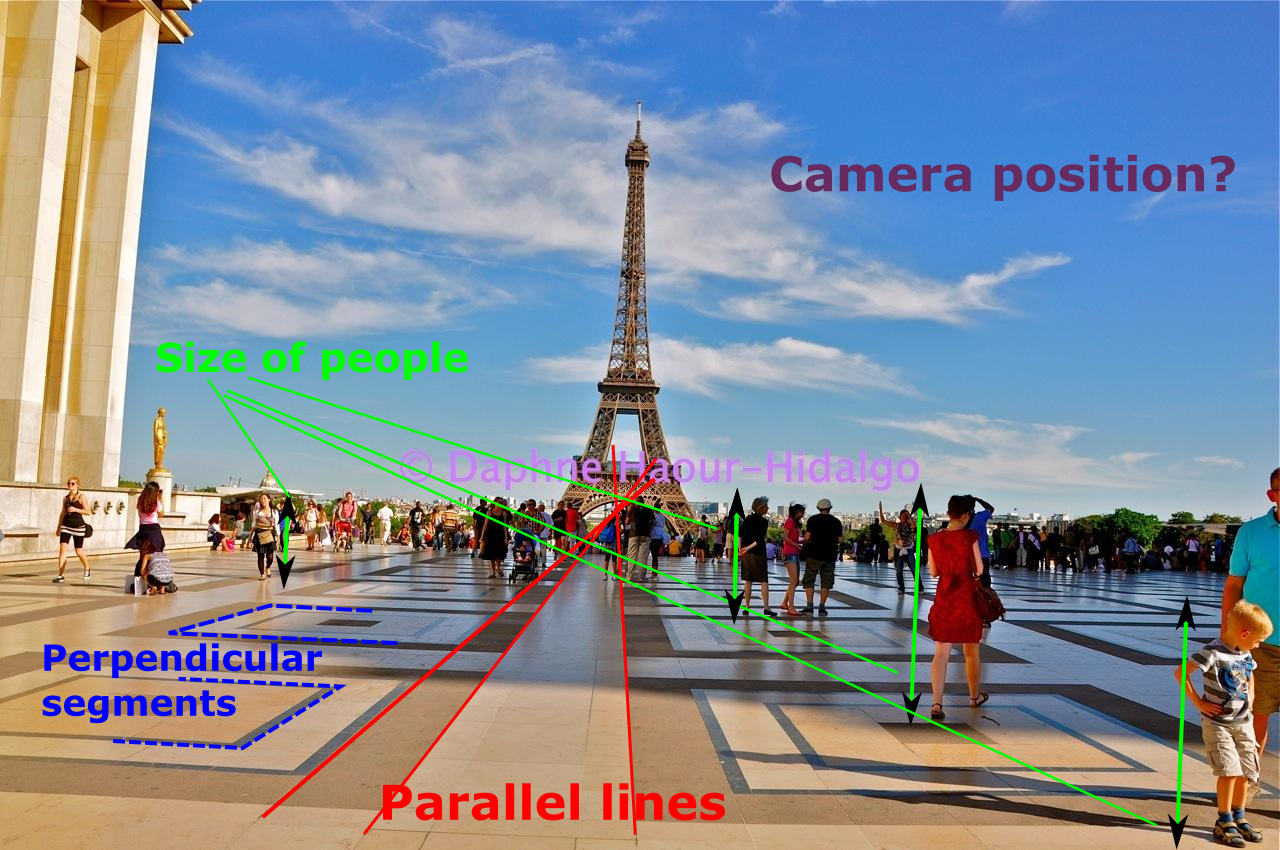
\includegraphics[width=0.8\textwidth]{IMAGES/trocadero_annotations}
  \end{center}
  Straight lines, connectivity, neighborhood.
\end{frame}


% ----------------------------------------------------
\begin{frame}
  \frametitle{Vanishing Points}
    \begin{center}
    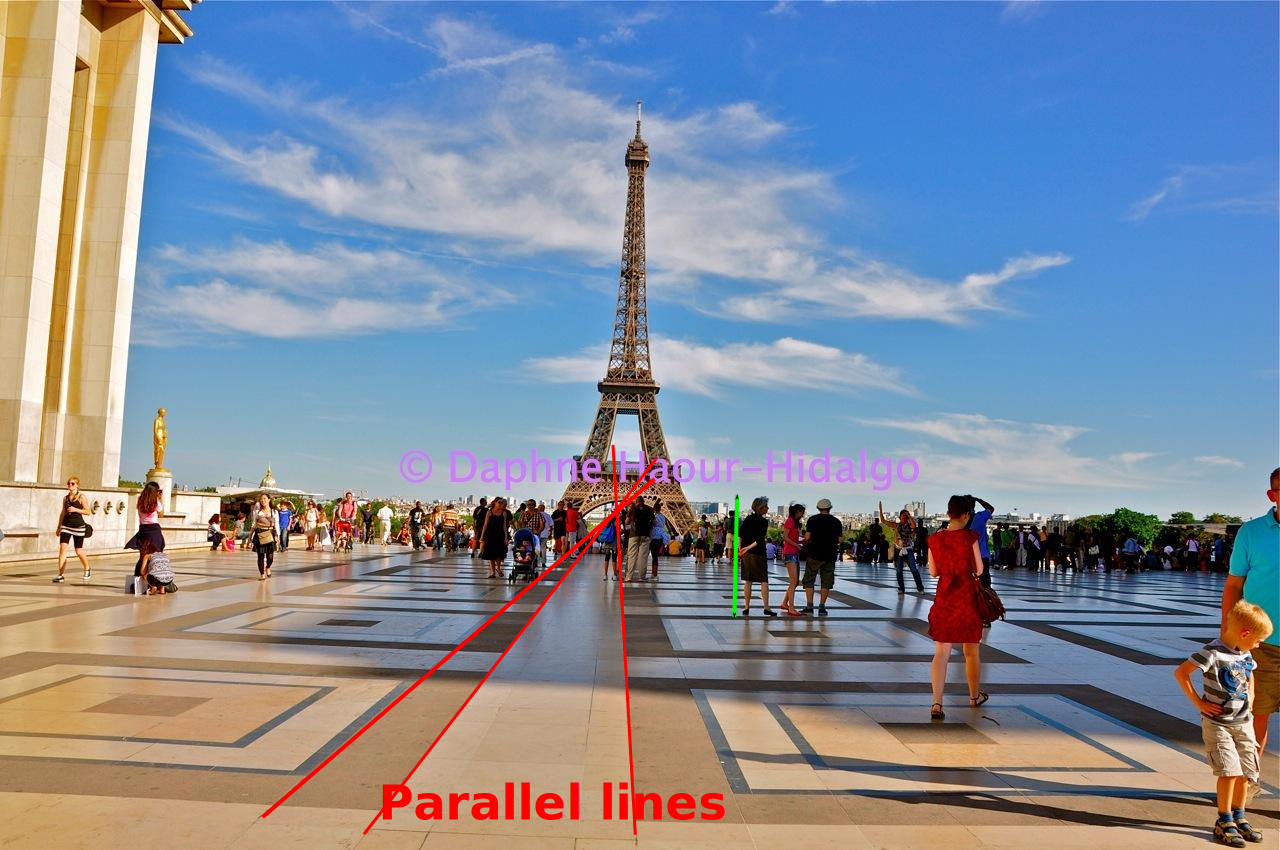
\includegraphics[width=0.8\textwidth]{IMAGES/trocaderolines}
  \end{center}
  Projections of parallel lines intersect at common points.
\end{frame}



% ----------------------------------------------------
\begin{frame}
\frametitle{Vanishing line}
  \begin{center}
    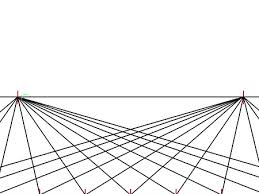
\includegraphics[width=0.4\textwidth]{IMAGES/vanishingline2.jpg}
    \hspace{2mm}
    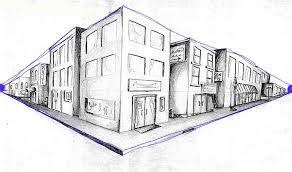
\includegraphics[width=0.4\textwidth]{IMAGES/vanishingline1.jpg}
  \end{center}
\end{frame}


% ----------------------------------------------------
\begin{frame}
  \frametitle{Exercises}
\begin{enumerate}
  \item  {\color{red}{How many vanishing points can there be in an
        image ?}} \\[3mm] 
       \pause    
       As many as there are planar sufaces with parallel linear
       texture \\[4mm]
  \item {\color{red}{Can we compute the vanishing line of a planar
        surface from images of 1, 2 or, 3 different sets of parallel
        lines on the surface?}} \\[3mm]
        \pause
        Yes, we need 2 sets of parallel lines.  This gives 2 VPs and
        the VL connecting them. \\[4mm]
   \item {\color{red}{May we compute 3D surface orientation (the
         surface normal)  from a vanishing line?}} \\[3mm]
      \pause
      Yes, if we know the focal length $f$ of the camera.  If the
      VL-equation is $Ax + By + C = 0$ then the 3D surface normal
      will be $(-\frac{f A}{C},  -\frac{f B}{C}, -1)$.
\end{enumerate}
\end{frame}



% ----------------------------------------------------
\begin{frame}
  \frametitle{Vanishing line}
  \begin{center}
    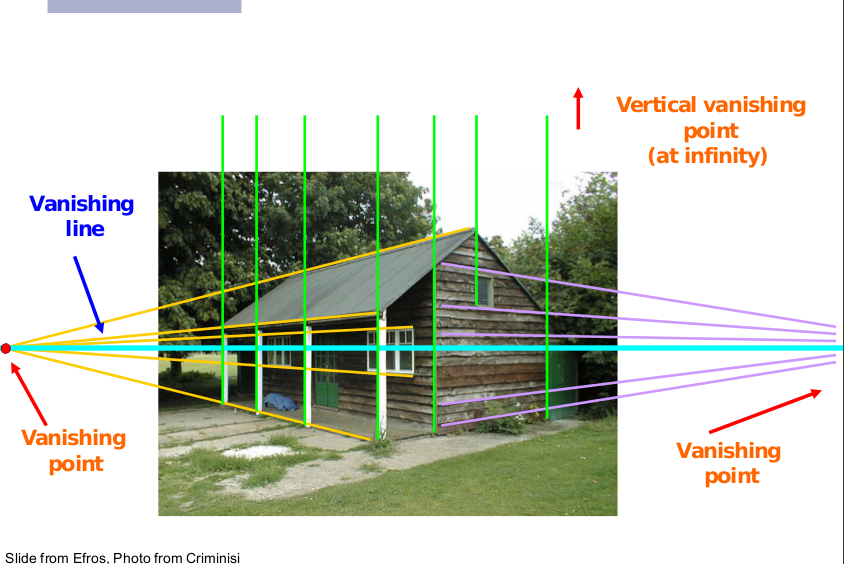
\includegraphics[width=0.8\textwidth]{FIGURES/vanishingline}
  \end{center}
\end{frame}



% ----------------------------------------------------
\begin{frame}
  \frametitle{VPs from texture}
    \begin{center}
      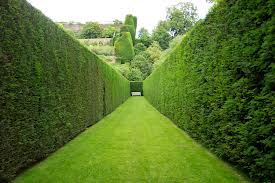
\includegraphics[width=0.65\textwidth]{IMAGES/hedges.jpg}
    \end{center}

If we can measure a texture density, then we may estimate the
directions of minimal and maximal density change. Theses points at the
VPs thus giving the VL and the 3D surface normal.
\end{frame}


% ----------------------------------------------------
\begin{frame}
  \frametitle{Homogeneous coordinates 1D}
  {\small
  \begin{itemize}
  \item In 1D coordinate is just 1 number. 
    \begin{center}
      
\includegraphics[width=0.75\textwidth]{FIGURES/1dcoords}
    \end{center}
  \item 1D coordinate to 1D Homogeneous coordinates: 
    $$x\sim
    \begin{bmatrix}
      x\\1
    \end{bmatrix}
    $$
  \item 1D homogeneous coordinate to 1 D coordinate
    $$
     \begin{bmatrix}
      x\\w
    \end{bmatrix}\sim x/w 
    $$
  \item What can we do with that? we can ``tame'' infinity!
  \item A point with homogeneous coordinate $[x,0]^T$ has ``normal'' coordinate $x/0 = \infty$
    as if we took homogeneous coordinate $[\infty,1]^T$
    \begin{center}
      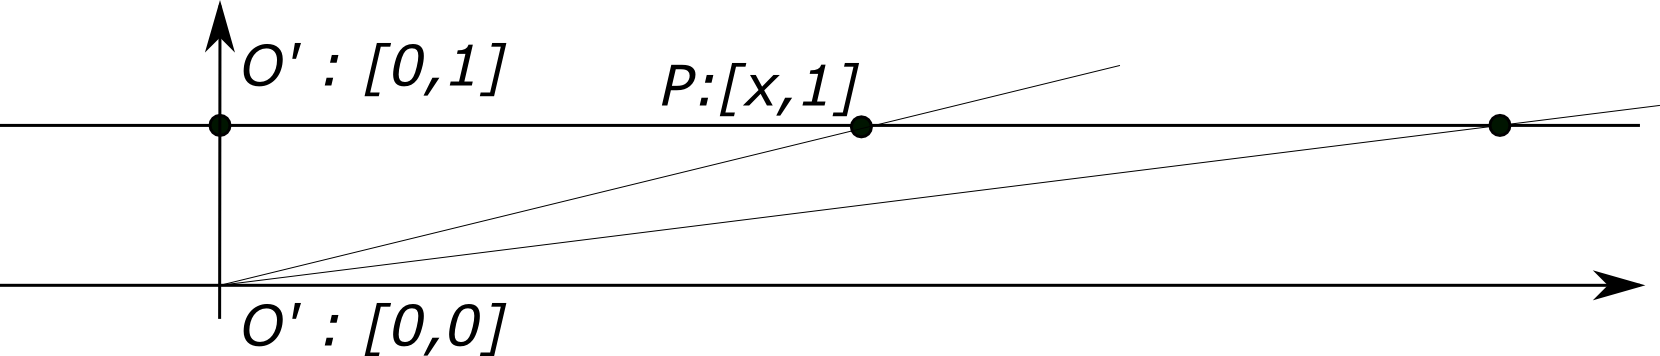
\includegraphics[width=0.75\textwidth]{FIGURES/1dcoordshomog}
    \end{center}
  \end{itemize}
  }
\end{frame}


% ----------------------------------------------------
\begin{frame}
  \frametitle{Homogeneous coordinates, 2D}
  ``Natural Coordinates'' for projective geometry
  \begin{itemize}
  \item From 2D point coordinate to 2D Homogeneous coordinate
    $$
    (x,y)\Implies
    \begin{bmatrix}
      x\\y\\1
    \end{bmatrix}
    $$
  \item From 2D homogeneous coordinates to 2D coordinates
    $$   
    \begin{bmatrix}
      x\\y\\w
    \end{bmatrix}
    \Implies 
    (x/w, y/w)
    $$
  % \item Exercise: Let $P$ have coordinates $(x,y,1)$ and let
  %   $Q(x',y',w)$ be a point on the line through $O (0,0,0)$ and $P$.  Compute $x'$ and $y'$.
  %   Considering $[x',y',w]$ as homogeneous 2D coordinates, what are
  %   the corresponding 2D coordinates?
  \end{itemize}
\end{frame}


% ----------------------------------------------------
\begin{frame}
  \frametitle{Homogeneous coordinates, 3D}
  \begin{itemize}
  \item From 3D point coordinate to 3D Homogeneous coordinate
    $$
    (x,y,z)\Implies
    \begin{bmatrix}
      x\\y\\z\\1
    \end{bmatrix}
    $$
  \item From 3D homogeneous coordinates to 3D coordinates
    $$   
    \begin{bmatrix}
      x\\y\\z\\w
    \end{bmatrix}
    \Implies 
    (x/w, y/w, z/w)
    $$
  \end{itemize}
\end{frame}


% ----------------------------------------------------
\begin{frame}
  \frametitle{Homogeneous coordinates}
  \begin{center}
    
\includegraphics[width=0.7\textwidth]{FIGURES/projcoords1}
  \end{center}
  Homogeneous coordinates in 2D correspond to points in plane $z=1$
  but also to lines through the origin and this point.
\end{frame}


% ----------------------------------------------------
\begin{frame}
  \frametitle{Why Are They Useful}
  \begin{itemize}
  \item Projection to image plane in standard coordinates:
    $$
    P: (x,y,z)\mapsto P': (f\frac{x}{z}, f\frac{y}{z})
    $$
  \item How does the mapping look like in homogeneous coordinates:\pause
    $$
    P:
    \begin{bmatrix}
      x\\y\\z\\1
    \end{bmatrix}
    \mapsto P': 
    \begin{bmatrix}
      fx\\fy\\z
    \end{bmatrix}
    $$
  \item Matrix notation
    $$
     \begin{bmatrix}
      fx\\fy\\z
    \end{bmatrix}
    = \udesc{K}{
    \begin{pmatrix}
      f & 0 & 0 & 0\\
      0 & f & 0 & 0\\
      0 & 0 & 1 & 0
    \end{pmatrix}}
    \begin{bmatrix}
      x\\y\\z\\1
    \end{bmatrix}
    $$
    \item $K$ is (a simple version of) the \myemph{Camera Calibration
        Matrix} and contains the intrinsic calibration parameters
      (here $f$).
  \end{itemize}
\end{frame}


% ----------------------------------------------------
\begin{frame}
  \frametitle{World, Camera and Image Coordinates}
  In the previous slides we were not precise on the many coordinate
  systems are implicitly used:\\[3mm] 
  \begin{itemize}
  \item 3D World Coordinates: Coordinate system of the 3D world. \\[3mm]
  \item Camera Coordinates: 3D coordinate system attached to the camera. \\[3mm]
  \item Image Coordinates: 2D Coordinate system attached to the image plane. \\[3mm]
  \item The coordinate system for the sampled and digitized image \\[3mm]
  \end{itemize}
  Not that simple in practice!
\end{frame}


% ----------------------------------------------------
\begin{frame}
  \frametitle{Assumptions Behind the Simple Model}
  \begin{center}
    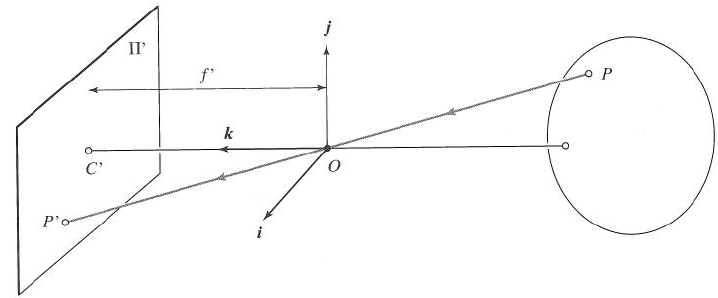
\includegraphics[width=0.8\textwidth]{FIGURES/fp14}
  \end{center}
  \begin{itemize}
    \item The camera center $0$ is the same as the world coordinates origin,
    \item The axes (base vectors) $\bi$, $\bj$ and $\bk$ are common
      for the camera and the world coordinate systems
    \item Pixels are squared and perfectly aligned with the camera coordinates
    \item Image coordinates have their origin at $C'$, projection of
      the camera center $O$ 
  \end{itemize}
\end{frame}


% ----------------------------------------------------
\begin{frame}
  \frametitle{Intrinsic vs Extrinsic Camera Parameters}
  Intrinsic parameters refer to {\color{blue}{internal parameters}}:
  \begin{itemize}
  \item Position of the image center wrt projection of the camera center: 2 parameters
  \item Scale factors (or sampling frequencies)  for the pixels sizes
    in both x and y directions: 2 parameters, 
  \item Skewness of pixels: 1 parameter.
  \end{itemize}
  {\color{blue}{Extrinsic Camera parameters}}:
  \begin{itemize}
  \item position of the camera coordinate system vs the world coordinates system:
    translation: 3 parameters,
  \item orientation of the camera coordinate system vs the world coordinates system:
    rotation: 3 parameters.
  \end{itemize}
\end{frame}


% ----------------------------------------------------
\begin{frame}
  \frametitle{Oriented and Translated Camera}
  \begin{center}
    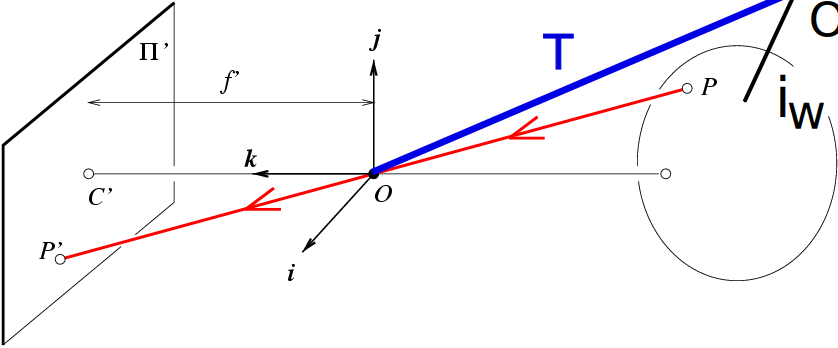
\includegraphics[width=0.9\textwidth]{FIGURES/orientedtranslatedcam1}
  \end{center}
\end{frame}


% ----------------------------------------------------
\begin{frame}
  \frametitle{Translating Coordinate System}
  \begin{center}
   
\includegraphics[width=0.5\textwidth]{FIGURES/translation3D} 
  \end{center}
%  Assume $O'$ at coordinates $(x_{O'},y_{O'},z_{O'})$ in coordinate system
%  $(O,\bi,\bj,\bk)$ and $P$ has coordinates $(x,y,z)$ also in $(O,\bi,\bj,\bk)$.
%  What are its coordinates in $(O',\bi,\bj,\bk)$?
% \end{frame}
%
%
% ----------------------------------------------------
% \begin{frame}  
  \begin{itemize}
%   \item Let $(x',y',z')$ its coordinates in $(O,\bi,\bj,\bk)$.
%   \item Write $\overrightarrow{O'P}$ = $\overrightarrow{OP} - \overrightarrow{OO'}$
%   \item Develop:
     \item Subtract the translation vector:
     $$
     \begin{pmatrix}
       x'\\y'\\z'
     \end{pmatrix}
     = 
     \begin{pmatrix}
       x\\y\\z
     \end{pmatrix}
     -
     \begin{pmatrix}
       x_{O'}\\y_{O'}\\z_{O'}
     \end{pmatrix}
     =
     \begin{pmatrix}
       x-x_{O'}\\y-y_{O'}\\z-z_{O'}
     \end{pmatrix}
     $$
   \item Transformation in homogeneous coordinates:
     $$
     \begin{bmatrix}
       x'\\y'\\z'\\1
     \end{bmatrix}
     =
     \begin{pmatrix}
       1 & 0 & 0 & -x_{O'}\\
       0 & 1 & 0 & -y_{O'}\\
       0 & 0 & 1 & -z_{O'}\\
       0 & 0 & 0 & 1
     \end{pmatrix}
     \begin{bmatrix}
       x\\y\\z\\1
     \end{bmatrix}
     $$
   \end{itemize}
 \end{frame}


% ----------------------------------------------------
 \begin{frame}
   \frametitle{Rotating Coordinate System}
   \begin{columns}
     \column{0.5\textwidth}
     \begin{center}
       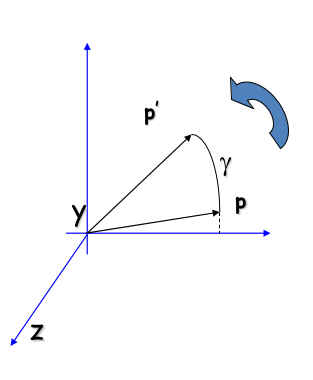
\includegraphics[width=\textwidth]{FIGURES/rotation3d}
     \end{center}
     \column{0.5\textwidth}
     Rotations along coordinate axes
     $$
     R_{x\alpha} = 
     \begin{pmatrix}
       1 & 0 & 0\\
       0 & \cos\alpha & -\sin\alpha\\
       0 & \sin\alpha & \cos\alpha
     \end{pmatrix}
     $$
     $$
     R_{y\beta} = 
     \begin{pmatrix}
       \cos\beta & 0 & -\sin\beta\\
       0 & 1 & 0\\
       \sin\beta & 0 & \cos\beta
     \end{pmatrix}
     $$
     $$ 
     R_{y\gamma} = 
     \begin{pmatrix}
       \cos\gamma & -\sin\gamma & 0\\
       \sin\gamma & \cos\gamma & 0\\
       0 & 0 & 1
     \end{pmatrix}
     $$
   \end{columns}~\\
   ~\\
   Can also be written in homogeneous coordinates
 \end{frame}
 

% ----------------------------------------------------
 \begin{frame}
   \frametitle{3D rotations}
To obtain a 3D rotation apply all 3 single-axis rotations:
{\small
\begin{eqnarray*}
     R &=&  R_{x\alpha}   R_{y\beta}  R_{y\gamma} \\[3mm]
        &=&
     \begin{pmatrix}
       1 & 0 & 0\\
       0 & \cos\alpha & -\sin\alpha\\
       0 & \sin\alpha & \cos\alpha
     \end{pmatrix}
     \;\;
     \begin{pmatrix}
       \cos\beta & 0 & -\sin\beta\\
       0 & 1 & 0\\
       \sin\beta & 0 & \cos\beta
     \end{pmatrix}
     \;\;
     \begin{pmatrix}
       \cos\gamma & -\sin\gamma & 0\\
       \sin\gamma & \cos\gamma & 0\\
       0 & 0 & 1
     \end{pmatrix} 
\end{eqnarray*}
}
\vspace{3mm}

Please notice that the order of the 3 rotation matrices do
matter. However, no matter which order $(\alpha, \beta, \gamma)$ may
be found such that the resulting 3D rotation is correct.
\end{frame}
 

% ----------------------------------------------------
 \begin{frame}
   \frametitle{Camera Matrix}
   \begin{itemize}
   \item Combine world vs camera coordinates with
   \item Simple Camera calibration matrix, now extended with
     Image plane transformation (axis scalings, shear, translation)
     $$
     {\bf C} = {\bf K} \left[{\bf  R}\,\, {\bf t}\right]
     $$
   \item ${\bf K}$$3\times 3$ matrix encoding the homogeneous transformations
     inside the camera. ${\bf K}$ specifies the \myemph{Intrinsic parameters}.
   \item $\left[{\bf R}\,\, {\bf t}\right]$ Concatenation of world
     coordinates rotation and origin translation to align camera and
     world coordinates.
   \end{itemize}
   $$
   w
   \begin{bmatrix}
     u\\b\\1
   \end{bmatrix}
   = \udesc{{\bf K}}{
     \begin{pmatrix}
       \alpha & s & u_0\\
       0 & \beta & v_0\\
       0 & 0 & 1
     \end{pmatrix}}
   \udesc{\left[{\bf R}\,\, {\bf t}\right]}{
     \begin{pmatrix}
       r_{11} & r_{12} & r_{13} & t_x\\
       r_{21} & r_{22} & r_{23} & t_y\\
       r_{31} & r_{32} & r_{33} & t_z\\
     \end{pmatrix}}
   \begin{pmatrix}
     x\\y\\z\\1
   \end{pmatrix}
   $$
 \end{frame}
 


%----------------------------------------------
\begin{frame}
\frametitle{Exercise}
\begin{itemize}
  \item {\color{red}{How many independent parameters are there to
        estimate in a camera calibration ?}} \\[3mm]
    \pause
     12: 6 intrinsic and 6 extrinsic (sometimes simplified to 3+6) \\[4mm]
  \item {\color{red}{May all calibration parameters be found using
        Linear algebra ?}} \\[3mm] 
    \pause
    No, they don't appear in a linear combinations. Some are
    multiplied together. 
\end{itemize}
\end{frame}
 


%----------------------------------------------
\begin{frame}
\frametitle{The geometric transformation between \\ 
  two images of a planar scene}
  \begin{itemize}
   \item The perspective projection of a planar scene surface is a
     non-linear transformation $(X,Y,Z) \longrightarrow (x,y)$ called 
     an \myemph{homography}:
     $$
  \begin{bmatrix}
       w x\\w y\\w
     \end{bmatrix}
     =
     \begin{pmatrix}
       h_{11} & h_{12} & h_{13} \\
       h_{21} & h_{22} & h_{23} \\
       h_{31} & h_{32} & h_{33} 
     \end{pmatrix}
     \begin{bmatrix}
       X\\Y\\Z\\
     \end{bmatrix}
     =
     H \cdot {\bf X}
     $$
   \item The transformation between two images is an homography.
  \item Homographies conserves straight lines, but not parallelism. 
  \item Two parallel lines intersect at infinity: after an homography
    they may intersect at finite distance. 
  \end{itemize}
\end{frame}





%----------------------------------------------
\begin{frame}
  An homography can accurately describe the stitching of images of a
  planar scene.  Non-planar scenes cannot be stitched correctly using
  homographies. 

  \begin{center}
    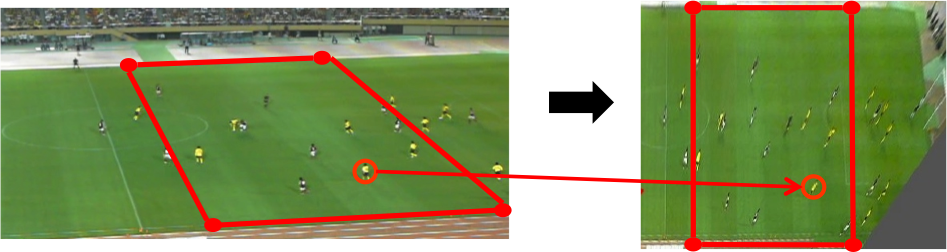
\includegraphics[width=0.85\textwidth]{MyImages/soccer_homography.png}
  \vspace{4mm}
    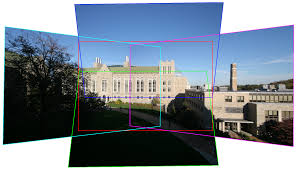
\includegraphics[width=0.6\textwidth]{MyImages/stitching.jpg}
  \end{center}
\end{frame}


% ----------------------------------------------------
 \begin{frame}
   \frametitle{Geometric Calibration}
   \begin{itemize}
     \item Computing the camera matrix is called geometric calibration.
     \item Extrinsic parameters: usually easy, but requires metric
       knowledge on scene features.
     \item Calibration focuses more on intrinsic parameters
       (calibration matrix ${\bf K}$): Some parameters are easy ($f$) and
       some ($(u_0, v_0)$) are difficult to estimate correctly.
   \end{itemize}
   \begin{columns}
     \column{0.5\textwidth}
     \begin{center}
       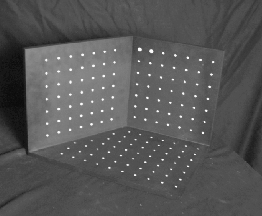
\includegraphics[width=0.8\textwidth]{IMAGES/calibrationobject}
     \end{center}
     \column{0.5\textwidth}
     \begin{itemize}
     \item Use an object with known geometry
     \item Use vanishing points / lines
     \item Use other cues...
     \end{itemize}
   \end{columns}
 \end{frame}


% ----------------------------------------------------
%  \begin{frame}
%   \begin{center}
%     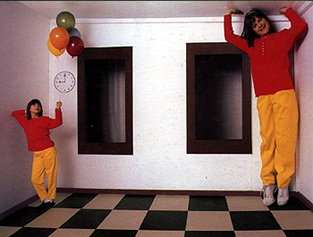
\includegraphics[width=0.8\textwidth]{IMAGES/amesroom}
%   \end{center}
%   Without knowledge of object geometry, calibration can be very problematic (Ames Room illusion).
% \end{frame}


% \section{More on Camera Models}


\begin{frame}
  \frametitle{Lens distortion}
  Cheap or wide-angle lenses causes geometric lens distortion. The
  most common distortion is (barral) radial distortion: 
  \begin{center}
  \begin{tabular}{c c c}
    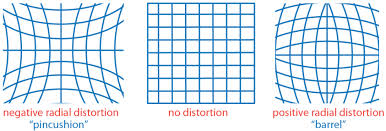
\includegraphics[width=0.55\textwidth]{MyImages/lensdistortion1.jpg}
    & \hspace{2mm} &
    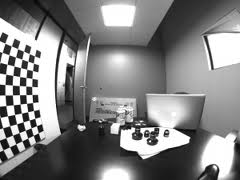
\includegraphics[width=0.3\textwidth]{MyImages/lensdistortion2.jpg}
   \end{tabular}
  \end{center}
  To comply with the assumptions of the pin-hole camera it may be
  necessary to correct for lens distortion before doing anything else.
\end{frame}


% ----------------------------------------------------
\begin{frame}
\frametitle{Lens distortion}
Lens distortion is non-linear.  The displacement of pixels may (for
radial distortion) be modeled as multiplicative even ordered
polynomium in radial distance from the principal point. \\[3mm]

% \begin{tabular}{r r}
%   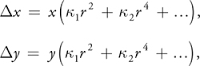
\includegraphics[width=0.5\textwidth]{MyImages/lensdistortion4.png}
\begin{minipage}{0.49\textwidth}
    \begin{eqnarray*}
      \Delta x  &=& x \left ( 
             \kappa_1 r^2 \;+\; \kappa_2 r^4 \;+\; \cdots \right ) \\
      \Delta y &=&  y \left ( 
             \kappa_1 r^2 \;+\; \kappa_2 r^4 \;+\; \cdots \right ) \\
      r^2  &= & x^2 + y^2 
      \end{eqnarray*}
\end{minipage}
% \hspace{2mm}
\begin{minipage}{0.50\textwidth}
    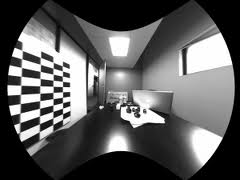
\includegraphics[width=0.50\textwidth]{MyImages/lensdistortion3.jpg}
\end{minipage}
%   \end{tabular}
%  \end{center}
\vspace{3mm}

Often only one or two terms are used.  The two konstants $\kappa_1$
and $\kappa_2$ are estimated using an iterative (nonlinear)
optimization approach.  
\end{frame}


% ----------------------------------------------------
% begin{frame}
%   \frametitle{Shrinking the aperture}
%   \begin{center}
%    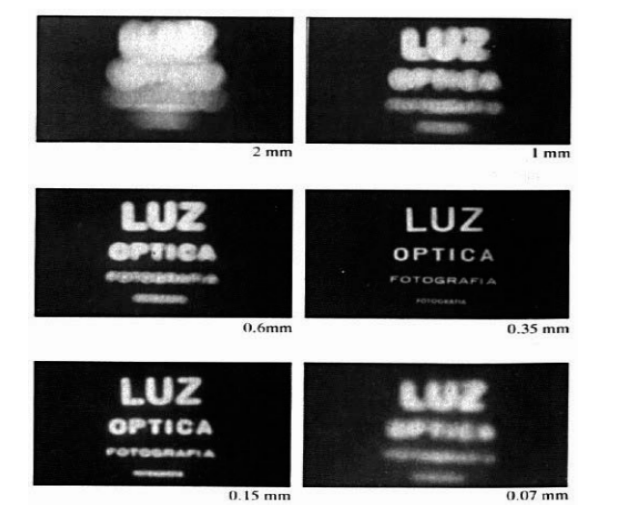
\includegraphics[width=0.7\textwidth]{IMAGES/shrinkingaperture}
%  \end{center}
%  Less light in, diffraction. 
% \end{frame}


% ----------------------------------------------------
\begin{frame}
  \frametitle{Focal Length, Aperture}
  \begin{center}
    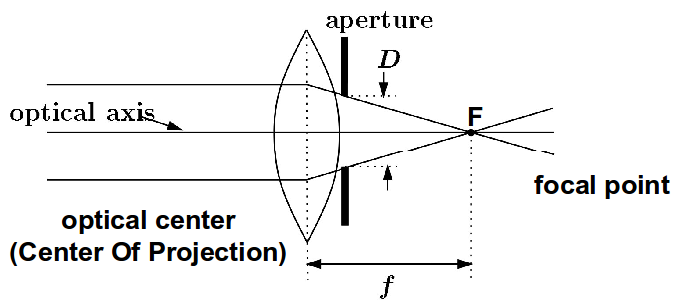
\includegraphics[width=0.8\textwidth]{FIGURES/focallength}
  \end{center}
  \begin{itemize}
  \item Lens focuses parallel rays into a single point.
  \item Aperture restricts range of rays.
  \item Zoom by ingreasing $f$, make wide angle by decreasing $f$
  \item In practice zoom optics use a set of lenses moving in a
    non-linear way wrt each other.
  \end{itemize}
\end{frame}


% ----------------------------------------------------
\begin{frame}
  \frametitle{Focus, Depth of Field}
   \begin{center}
    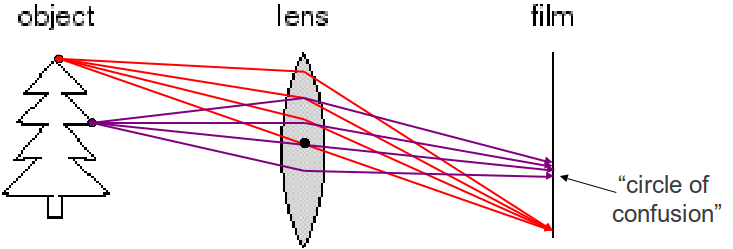
\includegraphics[width=0.7\textwidth]{FIGURES/addinglens}
  \end{center}
  \begin{itemize}
  \item Specific distance for which objects are in focus
  \item Changing shape of lens changes the focus distance.
  \item Changing distance between lens and sensor changes the 3D
    points in focus.
  \end{itemize}
\end{frame}


% ----------------------------------------------------
\begin{frame}
  \frametitle{The Eye is a Camera with Lens}
    \begin{center}
    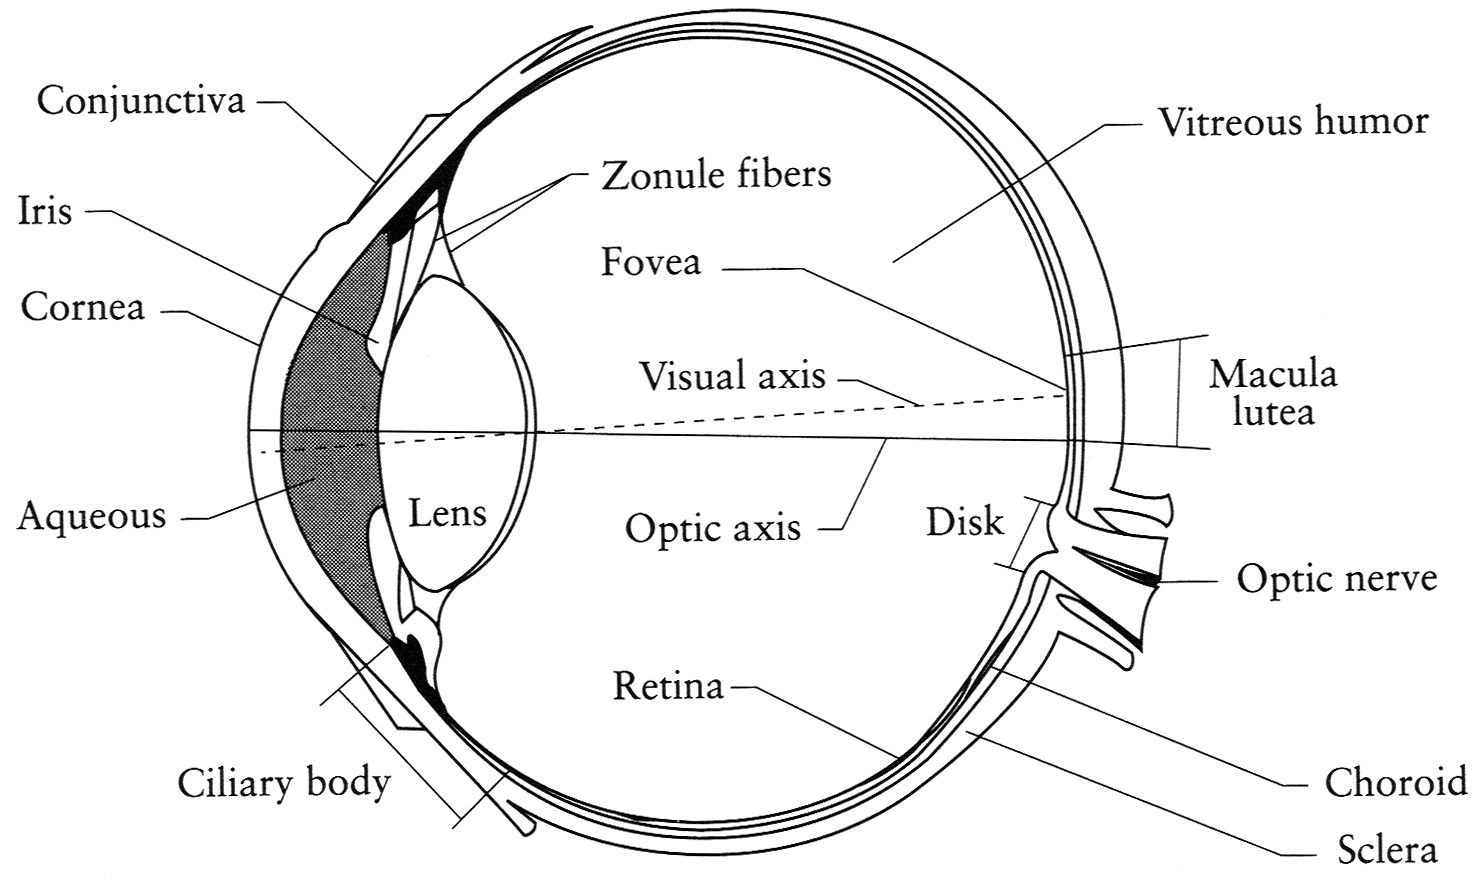
\includegraphics[width=0.9\textwidth]{FIGURES/theeye}
  \end{center}
\end{frame}


% ----------------------------------------------------
% \begin{frame}
%  \frametitle{Depth of Field}
%  \begin{center}
%    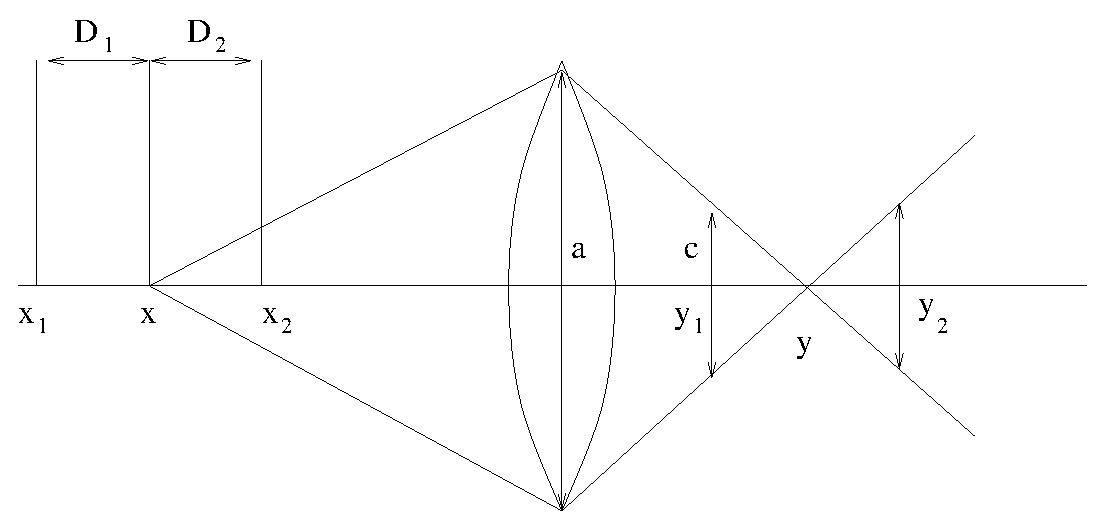
\includegraphics[width=0.6\textwidth]{FIGURES/depthoffield}
%  \end{center}
%  We shall later se that the Depth of field (DOF) is given by:
%  $$
%  DOF = \frac{2acfx(x-f)}{a^2f^2 - c^2x^2} \approx \frac{2cx^2}{af}
%  $$
%  where $a$ is the aperture, $f$ is the focal length, $c$ is the pixel
%  diameter, and $x$ is the distance. 
%  \begin{itemize}
%    \item To have a large DOF we would like large $c$ and $x$ and
%      small values of $f$ and $a$.
%    \item To estimate depth from focus we want a small DOF
%  \end{itemize}
%\end{frame}


% ----------------------------------------------------
% \begin{frame}
%  \frametitle{Depth from focus}
%  % \begin{center}
%    % 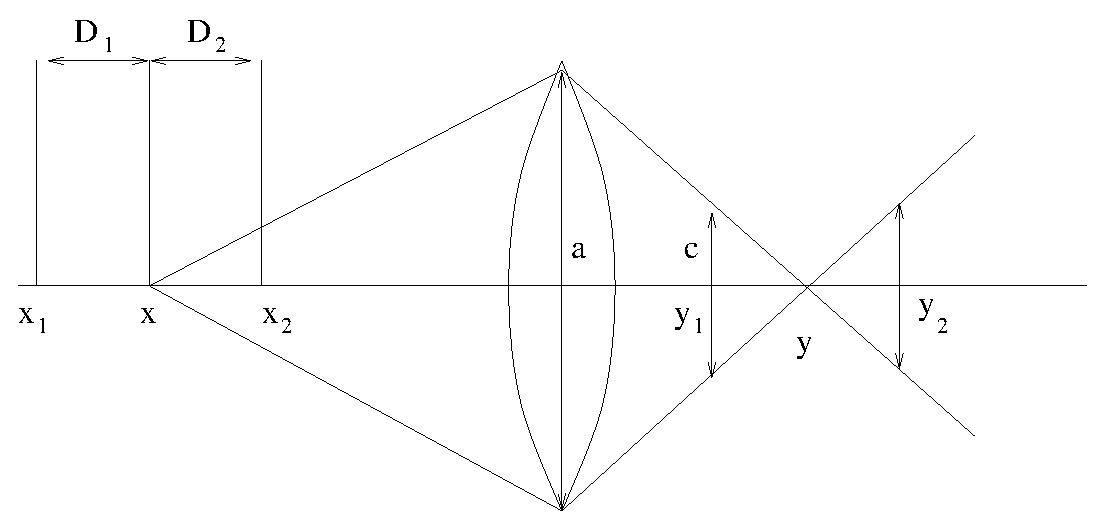
\includegraphics[width=0.9\textwidth]{FIGURES/depthoffield}
%  % \end{center}
%  A more realistic cemara model than the pin-hole model is the {\em
%    thin-lens} model. We shal later show that the equation for such a
%  lens is:
%  $$
%  \frac{1}{Z} + \frac{1}{d} = \frac{1}{f} 
%   \hspace{10mm}\mbox{or} \hspace{10mm}
%   Z  = \frac{fd}{d - f} 
%  $$  
%  where $f$ is the focal length and $d$ is the distance between the
%  lens and the image plane. 
%   \medskip
%
%  Thus, depth may be recovered from
%  knowledge of the focus setting that  brings things into focus. More
%  about this and Depth of field in a later lecture.
% \end{frame}


% ----------------------------------------------------
\begin{frame}
\frametitle{But we have two eyes}
    \begin{center}
    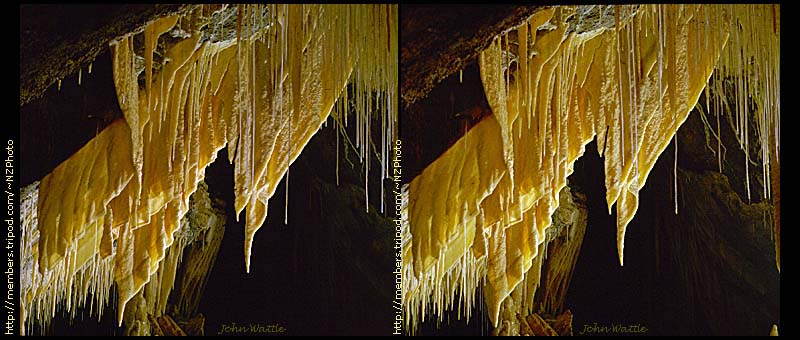
\includegraphics[width=0.9\textwidth]{MyImages/stereoEX1.jpg}
  \end{center}
Stereo vision is among the most important human sensing methods.
\medskip
Next Wednesday we will talk a lot about stereo vision.
\end{frame}



\end{document}


